\section{Phản ứng phân hạch - Phản ứng nhiệt hạch}
\subsection{Tóm tắt lí thuyết}
\begin{tomtat}
	\subsubsection{Phản ứng phân hạch}
	\paragraph{Khái niệm}
\begin{dn}
	Sự phân hạch là hiện tượng một hạt nhân rất nặng vỡ thành các hạt nhân nhẹ hơn.
\end{dn}
	\textbf{\textit{Ví dụ:}} Sự phân hạch của uranium 235 $\left(\ce{^{235}_{92}U}\right)$
	\begin{center}
		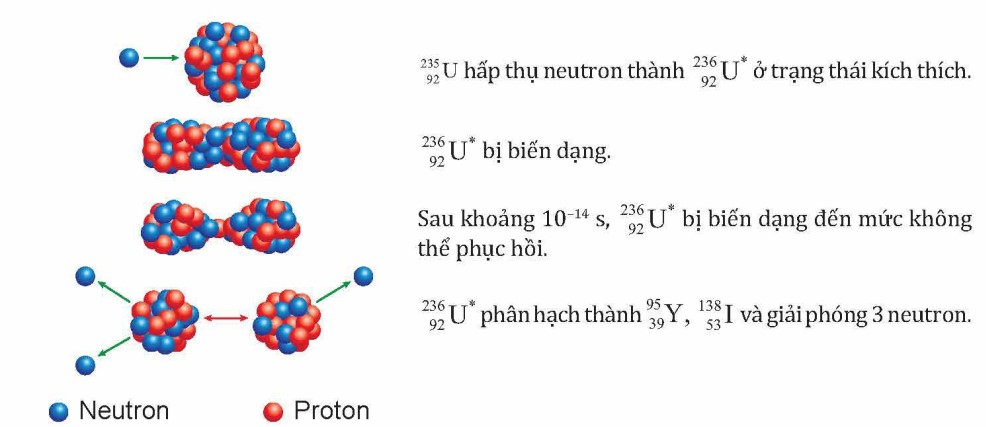
\includegraphics[width=0.7\linewidth]{figs/VN12-Y24-PH-SYL-030-1}
		\captionof{figure}{Tiến trình phân hạch của $\ce{^{235}_{92}U}$.}
	\end{center}
	Dùng một neutron nhiệt (còn gọi là neutron chậm) có động năng cỡ $\SI{0.01}{\electronvolt}$ bắn vào hạt nhân $\ce{^{235}_{92}U}$. Sau khi hấp thụ neutron nhiệt, $\ce{^{235}_{92}U}$ chuyển sang trạng thái kích thích $\ce{^{236}_{92}U}$. Trạng thái này không bền vững và kết quả là xảy ra quá trình phân hạch, $\ce{^{236}_{92}U}$ vỡ ra thành hai hạt nhân có số khối nhỏ hơn là $\ce{^{92}_{36}Kr}$ và $\ce{^{141}_{56}Ba}$, kèm theo 3 neutron. Phản ứng tạo ra một lượng năng lượng khoảng $\SI{200}{\mega\electronvolt}$ chủ yếu dưới dạng động năng của các hạt tạo thành.
	$$\ce{^{235}_{92}U}+\ce{^1_0n}\longrightarrow\ce{^{141}_{56}Ba}+\ce{^{92}_{36}Kr}+3\ce{^1_0n}.$$
	\paragraph{Hệ số nhân neutron - Phản ứng dây chuyền}
	\begin{dn}
		Hệ số nhân neutron $k$ là số neutron được sinh ra sau phản ứng hạt nhân trừ đi số neutron bị hấp thụ bởi môi trường xung quanh \textit{(hay số neutron trung bình còn lại sau mỗi phản ứng phân hạch)}.
	\end{dn}
	\begin{itemize}
		\item Nếu $k<1$: phản ứng dây chuyền không xảy ra.
		\item Nếu $k=1$: phản ứng dây chuyển tới hạn, mật độ neutron không đổi. Đây là phản ứng dây chuyển được sử dụng trong các lò phản ứng hạt nhân để tạo ra năng lượng.
		\item Nếu $k>1$: phản ứng dây chuyền vượt hạn, mật độ neutron tăng liên tục theo thời gian. Phản ứng dây chuyền không điều khiển được và xảy ra trong các vụ nổ hạt nhân.
	\end{itemize}
	\subsubsection{Phản ứng nhiệt hạch}
	\paragraph{Khái niệm}
	\begin{dn}
		Phản ứng tổng hợp hạt nhân (phản ứng nhiệt hạch) là quá trình trong đó hai hạt nhân nhẹ kết hợp với nhau để tạo thành hạt nhân nặng hơn. Phản ứng nhiệt hạch chỉ có thể xảy ra ở nhiệt độ cực cao.
	\end{dn}
	\textbf{\textit{Ví dụ:}} Phản ứng nhiệt hạch là nguồn gốc năng lượng của Mặt Trời và các ngôi sao, trong đó có sự tạo thành hạt nhân helium từ các hạt nhân hydrogen:
	$$4\ce{^1_1H}\longrightarrow \ce{^4_2He}+2\ce{^0_{+1}e^+}+\SI{26.8}{\mega\electronvolt}.$$
	\paragraph{Đặc điểm}
	\begin{itemize}
		\item Một phản ứng nhiệt hạch toả ra năng lượng nhỏ hơn một phản ứng phân hạch nhưng nếu tính theo khối lượng nhiêu liệu thì phản ứng nhiệt hạch toả năng lượng lớn hơn phản ứng phân hạch.
		\item Các phản ứng nhiệt hạch chỉ xảy ra ở nhiệt độ rất cao, khoảng 50 đến 100 triệu độ vì chỉ ở nhiệt độ cao thì các hạt nhân nhẹ mới thu được động năng đủ lớn thắng được lực đẩy Coloumb tiến lại gần nhau đến mức lực hạt nhân tác dụng kết hợp chúng lại.
		\item Năng lượng Mặt Trời và các sao có nguồn gốc từ các phản ứng nhiệt hạch.
		\item Con người đã tạo ra được phản ứng nhiệt hạch dạng không kiểm soát được (bom khinh khí).
		\item So với năng lượng phân hạch, năng lượng nhiệt hạch ưu việt hơn do nguồn nhiên liệu dồi dào, không gây ô nhiễm môi trường.
	\end{itemize}
	\subsubsection{Một số ngành công nghiệp hạt nhân trong đời sống}
	Công nghệ hạt nhân có một số ứng dụng thực tiễn như:
	\begin{itemize}
		\item Trong công nghiệp năng lượng: các nhà máy điện hạt nhân khai thác năng lượng từ các phản ứng phân hạch, phản ứng phân hạch tạo lực đẩy cho các phương tiện có công suất lớn (tên lửa, tàu ngầm, tàu phá băng, \dots) di chuyển.
		\item Trong y học: kiến thức vật lí hạt nhân được ứng dụng rộng rãi trong chẩn đoán và điều trị bệnh, đặc biệt là bệnh ung thư. Ví dụ hiệu ứng huỷ cặp electron - positron được ứng dụng trong máy chụp cắt lớp phát xạ positron (PET).
		\item Trong nông nghiệp: cải tạo giống cây trồng có các đặc tính mới: năng suất cao, chất lượng dinh dưỡng tốt, hình dáng đẹp, \dots
		\item Trong công nghiệp: kiểm tra chất lượng sản phẩm, đo mật độ vật liệu mà không phá huỷ mẫu vật, kiểm tra chất lượng mối hàn, \dots
		\item Trong khảo cổ: xác định tuổi và thành phần cấu tạo chất của các mẫu vật.
		\item Trong công nghệ thực phẩm: diệt vi sinh vật để khử trùng thực phẩm, làm chậm quá trình chín giúp trái cây được bảo quản lâu hơn ở điều kiện thường.
	\end{itemize}
\end{tomtat}
\subsection{Ví dụ minh hoạ}
\begin{dang}{Xác định năng lượng phản ứng phân hạch/ nhiệt hạch}
		Nếu lượng nhiên liệu là $\xsi{m}{\left(\gram\right)}$ thì số hạt nhân phản ứng là:
		$$N=\dfrac{m}{M}\cdot N_A.$$
		Năng lượng toả ra của 1 phản ứng là $\varepsilon$ thì năng lượng toả ra của $N$ phản ứng là:
		$$\Delta E=N\varepsilon.$$	
\end{dang}
\begin{vd}
Phân hạch một hạt nhân $\ce{^{235}U}$ sẽ toả ra năng lượng $\SI{200}{\mega\electronvolt}$. Khi phân hạch $\SI{1}{\gram}\ \ce{^{235}U}$ thì năng lượng toả ra bằng bao nhiêu?
\loigiai{Số hạt nhân $\ce{^{235}U}$ có trong $\SI{1}{\gram}$:
	$$N=\dfrac{m}{M}\cdot N_A=\dfrac{\left(\SI{1}{\gram}\right)}{\left(\SI{235}{\gram/\mole}\right)}\cdot\left(\SI{6.02E-23}{\mole^{-1}}\right)=\SI{2.56E21}{\text{hạt}}.$$	
	Năng lượng toả ra:
	$$E=N\varepsilon=\SI{2.56E21}{}\cdot\left(\SI{200}{\mega\electronvolt}\right)=\SI{5.12E23}{\mega\electronvolt}.$$}
\end{vd}
% ================================================
\begin{vd}
	Xét phản ứng phân hạch: $\ce{^1_0n}+\ce{^{235}_{92}U}\longrightarrow \ce{^{95}_{42}Mo}+\ce{^{139}_{57}La}+2\ce{^1_0n}+7\ce{\beta^{-}}$. Biết mỗi hạt $\ce{^{235}_{92}U}$ phân hạch toả ra năng lượng $\SI{215}{\mega\electronvolt}$. Cho năng suất toả nhiệt của xăng là $\SI{4.6E7}{\joule/\kilogram}$ và $\SI{1}{\electronvolt}=\SI{1.6E-19}{\joule}$. Để có năng lượng tương đương khi  $\SI{100}{\gram}\ \ce{^{235}_{92}U}$ phân hạch hoàn toàn thì khối lượng xăng cần đem đốt bằng bao nhiêu?
	\loigiai{
	Số hạt nhân $\ce{^{235}U}$ có trong $\SI{100}{\gram}$ nhiên liệu:
	$$N=\dfrac{m}{M}\cdot N_A=\dfrac{\left(\SI{100}{\gram}\right)}{\left(\SI{235}{\gram/\mole}\right)}\cdot\left(\SI{6.02E23}{\mole^{-1}}\right)=\SI{2.56E23}{\text{hạt}}.$$
	Năng lượng toả ra khi phân hạch $\SI{100}{\gram} \ce{^{235}U}$:
	$$\Delta E=N\varepsilon=\SI{2.56E23}{}\cdot\left(\SI{215}{\mega\electronvolt}\right)=\SI{5.5E25}{\mega\electronvolt}\approx\SI{8.81E12}{\joule}.$$
	Khối lượng xăng cần dùng để tạo ra được năng lượng như trên:
	$$m=\dfrac{\Delta E}{q}=\SI{1.916E5}{\kilogram}.$$	
	}
\end{vd}
% ====================================
\begin{vd}
	Xét phản ứng nhiệt hạch: $\ce{^2_1D}+\ce{^2_1D}\longrightarrow \ce{^4_2 He}$. Cho $m_{\ce{D}}=\SI{2.0136}{u}$ và $m_{\ce{He}}=\SI{4.0015}{u}$; $\SI{1}{u}=\SI{931.5}{\mega\electronvolt/c^2}$. Biết năng suất toả nhiệt của thuốc nổ TNT là $\SI{4E3}{\joule/\kilogram}$; $\SI{1}{\electronvolt}=\SI{1.6E-19}{\joule}$. Để có năng lượng tương đương với $\SI{0.5}{\kilogram}\ \ce{^4_2He}$ tạo thành thì cần khối lượng TNT bằng bao nhiêu?
	\loigiai{
	Năng lượng toả ra của 1 phản ứng:
	$$\varepsilon=\left(2m_{\ce{D}}-m_{\ce{He}}\right)c^2=\SI{23.93955}{\mega\electronvolt}.$$
	Số hạt nhân $\ce{He}$ chứa trong $\SI{500}{\gram}\ \ce{^4_2He}$ tạo thành:
	$$N=\dfrac{m}{m_{\ce{He}}}=\dfrac{\left(\SI{0.5}{\kilo\gram}\right)}{4,0015\cdot\left(\SI{1.66055E-27}{\kilogram}\right)}=\SI{7.525E25}{\text{hạt}}.$$
	Năng lượng toả ra khi tạo thành $\SI{0.5}{\kilogram}\ \ce{He}$:
	$$\Delta E=N\varepsilon=\SI{7.52E25}{}\cdot\left(\SI{23.93955}{\mega\electronvolt}\right)=\SI{1.8E27}{\mega\electronvolt}\approx\SI{288.2}{\mega\joule}.$$
	Khối lượng thuốc nổ TNT cần dùng:
	$$m=\dfrac{\Delta E}{q}=\dfrac{\SI{288.2E6}{\joule}}{\SI{4E3}{\joule/\kilogram}}=\SI{72.05E3}{\kilogram}	.$$
	}
\end{vd}
\begin{dang}{Giải được bài toán liên quan đến hiệu suất nhà máy điện hạt nhân}
	\end{dang}
\begin{vd}
Một nhà máy điện hạt nhân dùng nhiên liệu uranium $\ce{^{235}_{92}U}$ có công suất phát điện là $\SI{100}{\mega\watt}$. Biết hiệu suất của nhà máy là $\SI{20}{\percent}$ và một hạt nhân uranium $\ce{^{235}_{92}U}$ phân hạch thì toả ra năng lượng $\SI{3.2E-11}{\joule}$. Lấy $N_A=\SI{6.02E23}{\mole^{-1}}$ và khối lượng mol của $\ce{^{235}_{92}U}$ là $\SI{235}{\gram/\mole}$. Nếu nhà máy hoạt động liên tục thì lượng uranium $\ce{^{235}_{92}U}$ nhà máy cần dùng trong 365 ngày là bao nhiêu?
\loigiai{
Công suất phát điện của nhà máy $\calP_{\text{ci}}=\SI{100}{\mega\watt}$.\\
Công suất lò phản ứng:
$$H=\dfrac{\calP_\text{ci}}{\calP}\Rightarrow \calP=\dfrac{\calP_\text{ci}}{H}=\SI{500}{\mega\watt}.$$
Năng lượng phản ứng hạt nhân trong lò phản ứng trong thời gian 365 ngày:
$$E=\calP t=\left(\SI{500E6}{\watt}\right)\cdot365\cdot 24\cdot\left(\SI{3600}{\second}\right)=\SI{1.5768E16}{\joule}.$$
Khối lượng uranium cần dùng trong 365 ngày:
$$m=\dfrac{N}{N_A}M=\dfrac{E}{\varepsilon N_A}M=\dfrac{\left(\SI{1.5768E16}{\joule}\right)}{\left(\SI{3.2E-11}{\joule}\right)\cdot\left(\SI{6.02E23}{\mole^{-1}}\right)}\cdot\left(\SI{235}{\gram/\mole}\right)=\SI{192.35E3}{\gram}=\SI{192.35}{\kilogram}.$$	
}
\end{vd}
\subsection{Bài tập}
\subsubsection{Trắc nghiệm nhiều phương án lựa chọn}
\setcounter{ex}{0}
\Opensolutionfile{ans}[ans/VN12-Y24-PH-SYL-028P-TN]
% ===================================================================
\begin{ex}
	Phản ứng nhiệt hạch là
	\choice
	{sự biến đổi hạt nhân dưới tác dụng nhiệt}
	{sự phân rã của một hạt nhân thành những hạt nhân khác một cách tự phát}
	{phản ứng trong đó một hạt nhân nặng vỡ thành các hạt nhân nhẹ hơn}
	{\True phản ứng hạt nhân toả năng lượng}
	\loigiai{}
\end{ex}
% ===================================================================
\begin{ex}
	Trong các phát biểu sau về phản ứng phân hạch và phản ứng nhiệt hạch, có bao nhiêu phát biểu \textbf{đúng}?	
	\begin{enumerate}[label=(\arabic*)]
		\item Đều là phản ứng hạt nhân toả năng lượng.
		\item Đều là hiện tượng một hạt nhân nặng vỡ ra thành các hạt nhân nhẹ hơn.
		\item Đều là phản ứng tổng hợp hạt nhân.
		\item Đều xảy ra sự biến đổi hạt nhân.
	\end{enumerate}
	\choice
	{1}
	{\True 2}
	{3}
	{4}
	\loigiai{Các phát biểu đúng là (1) và (4)}
\end{ex}
% ===================================================================
\begin{ex}
	Trong một phản ứng hạt nhân, luôn có sự bảo toàn
	\choice
	{số proton}
	{\True số nucleon}
	{số neutron}
	{khối lượng}
	\loigiai{}
\end{ex}
% ===================================================================
\begin{ex}
	Phần lớn năng lượng giải phóng trong phản ứng phân hạch là
	\choice
	{năng lượng toả ra do phóng xạ của các mảnh}
	{động năng các neutron phát ra}
	{\True động năng của các mảnh}
	{năng lượng các photon của tia $\gamma$}
	\loigiai{}
\end{ex}
% ===================================================================
\begin{ex}
	Tìm câu \textbf{sai}. Những điều kiện cần phải có để tạo ra phản ứng hạt nhân dây chuyền là
	\choice
	{sau mỗi lần phân hạch, số neutron giải phóng phải lớn hơn hoặc bằng 1}
	{lượng nhiên liệu (uranium, plutonium) phải đủ lớn để tạo nên phản ứng dây chuyền}
	{\True nhiệt độ phải được đưa lên cao}
	{phải có nguồn tạo ra neutron}
	\loigiai{}
\end{ex}
% ===================================================================
\begin{ex}
	Nguồn gốc năng lượng của Mặt Trời là do
	\choice
	{\True các phản ứng nhiệt hạch xảy ra trong lòng nó}
	{các phản ứng phân hạch xảy ra trong lòng nó}
	{các phản ứng hoá học xảy ra trong lòng nó}
	{các phản ứng hạt nhân tự phát dây chuyền trong lòng nó}
	\loigiai{}
\end{ex}
% ===================================================================
\begin{ex}
	Phản ứng hạt nhân nào sau đây \textbf{không phải} là phản ứng nhiệt hạch?
	\choice
	{$\ce{_1^2H}+\ce{_1^2H} \longrightarrow\ce{_2^4He}$}
	{$\ce{_1^2H}+\ce{_3^6Li} \longrightarrow 2\ce{_2^4He}$}
	{\True $\ce{_2^4He}+\ce{_7^{14}N} \longrightarrow\ce{_8^{17}O}+\ce{_1^1H}$}
	{$\ce{_1^1H}+\ce{_1^3H} \longrightarrow\ce{_2^4He}$}
	\loigiai{}
\end{ex}
% ===================================================================
\begin{ex}
	Tìm phát biểu \textbf{sai}.
	\choice
	{Phản ứng nhiệt hạch là sự tổng hợp hai hạt nhân nhẹ thành hạt nhân nặng hơn, còn phản ứng phân hạch là sự phá vỡ một hạt nhân nặng thành hai hạt nhân nhẹ hơn}
	{Năng lượng toả ra trong phản ứng nhiệt hạch lớn hơn năng lượng toả ra trong phản ứng phân hạch}
	{Phản ứng phân hạch và phản ứng nhiệt hạch đều là phản ứng hạt nhân toả năng lượng}
	{\True Hiện nay con người đã kiểm soát được phản ứng phân hạch và phản ứng nhiệt hạch}
	\loigiai{
		Hiện nay con người mới kiểm soát được phản ứng phân hạch trong lò phản ứng hạt nhân; còn với phản ứng nhiệt hạch thì mới chỉ thực hiện được phản ứng dưới dạng không kiểm soạt được (bom H).
	}
\end{ex}
% ===================================================================
\begin{ex}
	Hạt nhân $\ce{_{92}^{234}U}$ phát ra hạt $\ce{_2^4\alpha}$ và biến đổi thành hạt nhân mới, phương trình phản ứng của quá trình này có dạng
	\choice
	{$\ce{_{92}^{234}U} \rightarrow\ce{_2^4\alpha}+\ce{_{90}^{232}U}$}
	{\True $\ce{_{92}^{234}U} \rightarrow\ce{_2^4\alpha}+\ce{_{90}^{230}Th}$}
	{$\ce{_{92}^{234}U} \rightarrow\ce{_2^4\alpha}+ \ce{_{88}^{230}Th}$}
	{$\ce{_{92}^{234}U} \rightarrow\ce{_2^4\alpha}+ \ce{_{88}^{230}U}$}
	\loigiai{}
\end{ex}
% ===================================================================
\begin{ex}
	Một trong các phản ứng xảy ra trong lò phản ứng là:
	$$
	\ce{_0^1n}+\ce{_{92}^{235}U} \longrightarrow\ce{_{92}^{236}U} \longrightarrow\ce{_{57}^{143}La}+\ce{_{35}^{87}Br}+y\left(\ce{_0^1n}\right)
	$$
	với $y$ là số neutron. Giá trị $y$ bằng
	\choice
	{4}
	{\True 6}
	{8}
	{10}
	\loigiai{
		Áp dụng định luật bảo toàn số nucleon: $236=143+87+y\Rightarrow y=6.$
	}
\end{ex}
% ===================================================================
\begin{ex}
	Uranium $\left(\ce{^{235}U}\right)$ khi được kích thích bởi neutron chậm	sẽ phân hạch với phương trình phản ứng:
	$$\ce{^{235}_{92}U}+n\longrightarrow \ce{^{141}_{56}Ba}+\ce{^{92}_{y}Kr}+xn$$
	Các giá trị $x$ và $y$ lần lượt là
	\choice
	{\True $x=3$, $y=36$}
	{$x=3$, $y=34$}
	{$x=2$, $y=36$}
	{$x=2$, $y=35$}
	\loigiai{
		Bảo toàn điện tích và bảo toàn số khối ta được:
		$$\begin{cases}
			235+1=141+92+x\\
			92=56+y
		\end{cases}	\Rightarrow \begin{cases}
			x=3\\
			y=36
		\end{cases}.$$
	}
\end{ex}
% ===================================================================
\begin{ex}
	Uranium 238 là nguyên tố khởi đầu của một họ phóng xạ, cuối cùng cho ra đồng vị bền của chì $\ce{^{206}_{82}Pb}$. Các phân rã liên tục phát ra hạt $\alpha$ hoặc hạt $\beta^{-}$. Tuổi thọ của các hạt nhân trung gian khá ngắn để người ta có thể bỏ qua sự hiện diện của chúng. Như vậy, sự phân rã có thể thu gọn trong một phản ứng duy nhất:
	$$\ce{^{238}_{92}U}\longrightarrow \ce{^{206}_{82}Pb}+x\alpha+y\beta^-.$$ 
	Các giá trị $x$ và $y$ lần lượt là
	\choice
	{$x=5$, $y=12$}
	{$x=6$, $y=8$}
	{\True $x=8$, $y=6$}
	{$x=4$, $y=2$}
	\loigiai{
		$$\ce{^{238}_{92}U}\longrightarrow \ce{^{206}_{82}Pb}+x\ce{^4_2\alpha}+y\ce{^0_{-1}\beta^-}$$ 
		Bảo toàn điện tích và bảo toàn số khối ta được:
		$$
		\begin{cases}
			238=206+4x\\
			92=82+2x-y
		\end{cases}\Rightarrow \begin{cases}
			x=8\\
			y=6
		\end{cases}.
		$$	
	}
\end{ex}

% ===================================================================
\begin{ex}
	Xét phản ứng phân hạch uranium có phương trình:
	$$
	\ce{_{92}^{235}U}+\ce{n} \longrightarrow\ce{_{42}^{95}Mo}+\ce{_{57}^{139}La}+2 \ce{n}+7 \ce{^{-}e}
	$$
	Cho khối lượng các hat: $\ce{m}_{\ce{U}}=234,99 \ce{u} ; \ce{m}_{\ce{Mo}}=94,88 \ce{u} ; \ce{m}_{\ce{La}}=138,87 \ce{u} ; \ce{m}_{\ce{n}}=1,0087 \ce{u}$; $1 \ce{u}=931,5 \ce{MeV} / \ce{c}^2$. Bỏ qua khối lượng của electron. Năng lượng mà một phân hạch tỏa ra bằng	
	\choice
	{$\SI{215.34}{\mega\electronvolt}$}
	{$\SI{723.76}{\mega\electronvolt}$}
	{$\SI{723.37}{\mega\electronvolt}$}
	{\True $\SI{215.46}{\mega\electronvolt}$}
	\loigiai{
		$E=\left(m_{\ce{U}}+m_n-m_{\ce{Mo}}-m_{\ce{La}}-2m_n\right)c^2=\SI{0.2313}{u}c^2=\SI{215.46}{\mega\electronvolt}.$
	}
\end{ex}
% ===================================================================
\begin{ex}
	Cho rằng một hạt nhân uranium $\mathrm{_{92}^{235}U}$ khi phân hạch thì tỏa ra năng lượng là $\SI{200}{\mega\electronvolt}$. Năng lượng tỏa ra khi $\SI{2}{\gram}$ uranium $\mathrm{_{92}^{235}U}$ phân hạch hết là
	\choice
	{$\SI{9.6E10}{\joule}$}
	{$\SI{10.3E23}{\joule}$}
	{$\SI{16.4E23}{\joule}$}
	{\True $\SI{16.4E10}{\joule}$}
	\loigiai{
		Số hạt uranium có trong $\SI{2}{\gram}$: $N=\dfrac{2}{235}N_A=\SI{5.12E21}{\text{hạt}}$.\\
		Năng lượng tỏa ra: $$E=200N=\SI{1.025E24}{\mega\electronvolt}=\SI{16.4E10}{\joule}.$$
	}
\end{ex}
% ===================================================================
\begin{ex}
	Xét lần lượt hai phản ứng sau:
	\begin{itemize}
		\item \textbf{Phản ứng 1:} $\ce{_{92}^{235}U}+\ce{_0^1n} \longrightarrow\ce{_{60}^{143}Nd}+\ce{_{40}^{90}Zr}+3\ce{_0^1n}+8\ce{_{-1}^0e}+8 \bar{v}_{e}+\SI{200}{\mega\electronvolt}$. Khối lượng của $\ce{_{92}^{235}U}$ sử dụng trong phản ứng 1 là $\SI{50}{\gram}$.
		\item \textbf{Phản ứng 2:} $\ce{_1^1H}+\ce{_0^1n} \longrightarrow \ce{_1^2D}+\SI{2.23}{\mega\electronvolt}$. Khối lượng $\ce{_1^2D}$ tạo thành từ phản ứng 2 là $\SI{50}{\gram}$.	
	\end{itemize}
	Biết số Avogadro là $N_{A} \approx \SI{6.022E23}{\mole^{-1}}$.
	Nhận định nào sau đây \textbf{đúng}?
	\choice
	{Phản ứng 1 thuộc loại phản ứng nhiệt hạch, năng lượng toả ra khi phản ứng hết $\SI{50}{\gram}\ \ce{_{92}^{235}U}$ là $\SI{2.56E25}{\mega\electronvolt}$}
	{Phản ứng 2 thuộc loại phản ứng phân hạch, năng lượng toả ra khi thu được $\SI{50}{\gram}\  \ce{_1^2D}$ là $\SI{3.36E25}{\mega\electronvolt}$}
	{Xét về năng lượng toả ra của một phản ứng thì phản ứng nhiệt hạch có giá trị lớn hơn phản ứng phân hạch}
	{\True Tổng năng lượng toả ra ở phản ứng 2 lớn gấp 1,3125 lần tổng năng lượng toả ra ở phản ứng 1}
	\loigiai{
		Năng lượng tỏa ra khi sử dụng hết $\SI{50}{\gram}\ \ce{^{235}_{92}U}$:
		$$Q_1=\dfrac{50}{235}\cdot\SI{6.022E23}{}\cdot200\approx\SI{2.56E25}{\mega\electronvolt}.$$
		Năng lượng tỏa ra khi thu được $\SI{50}{\gram}\ \ce{^2_1D}$:
		$$Q_2=\dfrac{50}{2}\cdot\SI{6.022E23}\cdot2,23\approx\SI{3.36E25}{\mega\electronvolt}$$
		Vậy năng lượng tỏa ra ở phản ứng nhiệt hạch lớn hơn phản ứng phân hạch nói trên 1,3125 lần trong các trường hợp đang xét.
	}
\end{ex}
% ===================================================================
\begin{ex}
	Bom hydrogen (bom $\ce{H}$) là một loại vũ khí hạt nhân có sức tàn phá lớn hơn bom nguyên tử (bom A) rất nhiều lần, dù hiện nay cả bom hydrogen và bom nguyên tử đều không được sử dụng trong các cuộc chiến tranh. Sở dĩ bom hydrogen có sức tàn phá lớn như vậy là do nó là sự kết hợp của phản ứng phân hạch của $\ce{_{92}^{235}U}$ (giai đoạn 1) để tạo ra môi trường có nhiệt độ rất cao, cung cấp động năng cho các hạt tham gia phản ứng nhiệt hạch (giai đoạn 2) theo phương trình phản ứng $\ce{_1^2H}+\ce{_1^3H} \longrightarrow\ce{_2^4He}+ \ce{_0^1n}+\SI{17.6}{\mega\electronvolt}$. Giả sử năng lượng toả ra từ quá trình phân hạch còn lại sau khi tạo phản ứng nhiệt hạch là $\SI{2.8E10}{\joule}$ và khối lượng $\ce{_2^4 He}$ được tạo thành từ một vụ nổ bom hydrogen trong thí nghiệm vũ khí hạt nhân là $\SI{200}{\gram}$ thì sức tàn phá của quả bom này tương đương với khoảng bao nhiêu tấn thuốc nổ TNT? Biết rằng năng lượng toả ra khi một tấn thuốc nổ TNT cháy hoàn toàn là $\SI{4.2E9}{\joule}$. Cho số Avogadro là $N_{A}=\SI{6.022e23}{\mole^{-1}}$.
	\choice
	{\True 20197,14 tấn}
	{20190,48 tấn.}
	{20166,6 tấn.}
	{20183,81 tấn}
	\loigiai{
		số lượng $\ce{_2^4He}$ được tạo thành là:
		$$
		N_{\ce{He}}=\dfrac{200}{4} \cdot 6,022 \cdot 10^{23}=\SI{3.011E25}{\text{hạt}}
		$$
		Tổng năng lượng toả ra của các phản ứng nhiệt hạch là:
		$$
		Q=3,011 \cdot 10^{25} \cdot\left(17,6 \cdot 10^6 \cdot 1,6 \cdot 10^{-19}\right) \approx \SI{8.48E13}{\joule}
		$$
		Khối lượng thuốc nổ TNT cần dùng để năng lượng toả ra tương đương với bom hydrogen là:
		$$
		m=\dfrac{2,8 \cdot 10^{10}+8,48 \cdot 10^{13}}{4,2 \cdot 10^9} \approx \SI{20197.14}{\text { tấn }}
		$$
	}
\end{ex}
\Closesolutionfile{ans}
\subsubsection{Trắc nghiệm đúng/sai}
\Opensolutionfile{ans}[ans/VN12-Y24-PH-SYL-028P-TF]
\setcounter{ex}{0}
% ===================================================================
\begin{ex}
	Trong mỗi phát biểu sau, em hãy chọn đúng hoặc sai.	
	\choiceTFt
	{Trong các phản ứng hạt nhân, điện tích và số khối được bảo toàn nên số neutron cũng được bảo toàn}
	{\True Cho phản ứng hạt nhân $\ce{_0^1n}+\ce{_{92}^{235}U} \longrightarrow\ce{_{38}^{94}Sr}+\ce{X}+2\ce{_0^1n}$. Hạt nhân $\ce{X}$ có 54 proton và 86 neutron}
	{Trong phản ứng nhiệt hạch: $\ce{_1^2H}+\ce{_1^3H} \longrightarrow \ce{_2^4He}+\ce{_0^1n}+\SI{17.6}{\mega\electronvolt}$, năng lượng cần cung cấp cho phản ứng là $\SI{17.6}{\mega\electronvolt}$}
	{\True Công nghệ hạt nhân đang được ứng dụng nhiều trong y học, công nghiệp, nông nghiệp, khảo cổ học, thực phẩm}
	{Trong phản ứng hạt nhân chỉ có sự bảo toàn điện tích và bảo toàn số khối}
	{\True Phản ứng nhiệt hạch là nguồn năng lượng của Mặt Trời và các sao}
	\loigiai{}
\end{ex}
% ===================================================================
\begin{ex}
	Hình bên là sơ đồ minh họa cho phản ứng tổng hợp hạt nhân thường xảy ra trên Mặt Trời và các ngôi sao.
	\begin{center}
		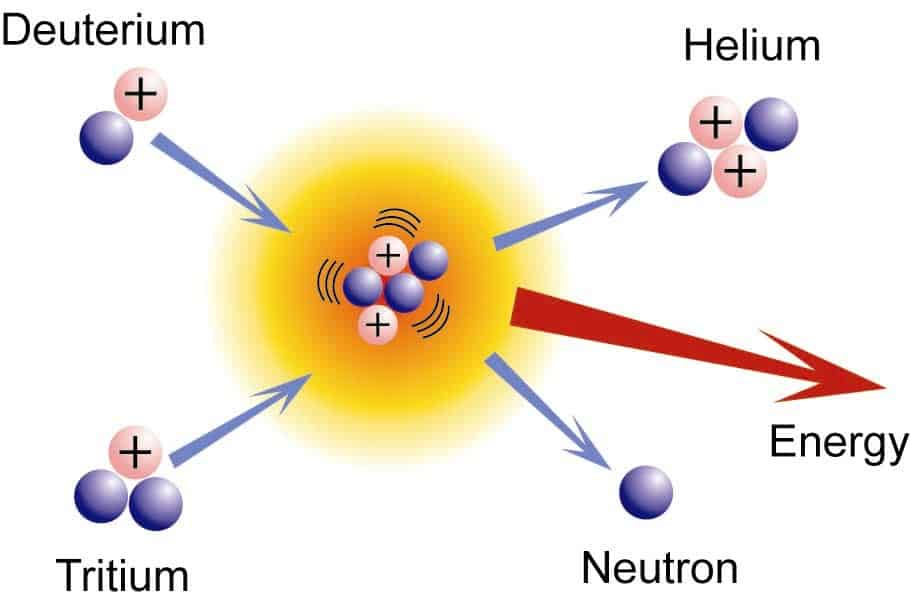
\includegraphics[width=0.35\linewidth]{figs/VN12-Y24-PH-SYL-030P-1}
	\end{center}
	\choiceTF[t]
	{\True Phản ứng này còn được gọi là phản ứng nhiệt hạch}
	{Đây là phản ứng thu năng lượng}
	{Phản ứng này tạo ra nhiều sản phẩm có tính phóng xạ}
	{Hiện nay, con người đã điều khiển được phản ứng này}
	\loigiai{
		\begin{itemchoice}
			\itemch Đúng.
			\itemch Sai. Đây là phản ứng tỏa năng lượng.
			\itemch Sai. Hiện trong các phản ứng tổng hợp hạt nhân chưa thấy hạt sản phẩm có tính phóng xạ.
			\itemch Sai. Con người chưa điều khiển được phản ứng nhiệt hạch.
		\end{itemchoice}
	}
\end{ex}
% ===================================================================
\begin{ex}
	Trái bom "Little Boy" mà Mỹ ném xuống thành phố Hiroshima của Nhật Bản ngày 6 tháng 8 năm 1945 chứa $\SI{60}{\kilogram}$ đồng vị uranium là $\ce{^{235}_{92}U}$. Coi như mỗi phản ứng phân hạch uranium tỏa năng lượng khoảng $\SI{200}{\mega\electronvolt}$.
	\choiceTF[t]
	{Người ta tạo ra phản ứng phân hạch dây chuyền có kiểm soát với hệ số nhân neutron bằng 1 để kích hoạt bom nổ}
	{\True Người ta tạo ra phản ứng phân hạch dây chuyền với hệ số nhân neutron lớn hơn 1 để kích hoạt bom nổ}
	{\True Phản ứng này đã tạo ra rất nhiều hạt phóng xạ gây nguy hiểm cho cơ thể con người một thời gian rất dài sau đó}
	{Để tạo ra năng lượng tương đương với quả bom thì cần 1,23 ngàn tấn thuốc nổ. Biết $\SI{1}{\kilogram}$ thuốc nổ tạo ra năng lượng $\SI{4E6}{\joule}$. Lấy khối lượng uranium bằng số khối của nó}
	\loigiai{
		\begin{itemchoice}
			\itemch Phản ứng dây chuyển trong bom không kiểm soát được, hệ số nhân neutron >1.
			\itemch Đúng.
			\itemch Đúng.
			\itemch Sai. Lượng thuốc nổ cần dùng là xấp xỉ 1,23 triệu tấn.
		\end{itemchoice}
	}
\end{ex}
% ===================================================================
\begin{ex}
	Trong một lò phản ứng hạt nhân sử dụng đồng vị phóng xạ $\ce{^{235}U}$, người ta dùng các neutron có động năng cỡ $\SI{0.01}{\electronvolt}$ bắn vào hạt nhân $\ce{^{235}U}$ để tạo ra phản ứng phân hạch: $\ce{n}+\ce{^{235}U}\longrightarrow\ce{X}+\ce{Y}+k\ce{n}+Q$. Trong đó $Q$ là năng lượng của quá trình phân hạch có giá trị khoảng $\SI{190}{\mega\electronvolt}$ bao gồm:
	\begin{itemize}
		\item nhiệt năng sinh ra: $\SI{167}{\mega\electronvolt}$;
		\item năng lượng neutron nhanh: $\SI{5}{\mega\electronvolt}$;
		\item bức xạ $\gamma$ tức thời: $\SI{7}{\mega\electronvolt}$;
		\item phát xạ beta của sản phẩm sau phân hạch: $\SI{5}{\mega\electronvolt}$;
		\item phát xạ $\gamma$ của các sản phẩm phân hạch: $\SI{6}{\mega\electronvolt}$.
	\end{itemize}
	\choiceTF[t]
	{\True Để lò hoạt động bình thường cần duy trì số neutron còn lại sau mỗi phân hạch bằng 1}
	{Các neutron sinh ra sau mỗi phản ứng sẽ tham gia ngay vào phản ứng tiếp theo mà không cần trải qua quá trình nào khác}
	{\True Nhiệt năng sinh ra trong mỗi phản ứng xấp xỉ $\SI{88}{\percent}$ năng lượng của phản ứng}
	{\True Để thu được công suất $\SI{100}{\mega\watt}$ từ nhiệt năng thì lượng $\ce{^{235}U}$ cần thiết trong 1 ngày là $\SI{126.2}{\gram}$}
	\loigiai{
		\begin{itemchoice}
			\itemch Đúng. Để duy trì phản ứng hạt nhân kiểm soát được, hệ số nhân neutron phải bằng 1.
			\itemch Sai. Các neutron sinh ra sau các phản ứng là các neutron nhanh, chúng cần được làm chậm để tham gia vào các phản ứng tiếp theo.
			\itemch Đúng. Tỉ lệ nhiệt năng so với năng lượng phản ứng: $p=\dfrac{167}{190}\approx\SI{88}{\percent}$.
			\itemch Đúng. Khối lượng $\ce{^{235}U}$ cần sử dụng: $m=\dfrac{100\cdot10^4\cdot24\cdot3600}{167\cdot\SI{1.6E-13}{}}\cdot\dfrac{235}{\SI{6.02E23}{}}=\SI{126.2}{\gram}.$
		\end{itemchoice}
	}
\end{ex}
\Closesolutionfile{ans}
\subsubsection{Tự luận}
\Opensolutionfile{ans}[ans/VN12-Y24-PH-SYL-028P-TL]
\setcounter{ex}{0}
% ======================================================================
\begin{ex}
	Xét phản ứng nhiệt hạch: $\ce{_1^2H}+\ce{_1^3H} \rightarrow \ce{_2^4He}+ \ce{_0^1}$. Để tổng hợp được $\SI{50}{\gram}$ hạt $\ce{\alpha}$ thì khối lượng $\ce{_1^2H}$ và $\ce{_1^3H}$ phải sử dụng là bao nhiêu? Coi khối lượng mol gần bằng số khối của hạt nhân. Biết số Avogadro là $N_{A} \approx \SI{6.022E23}{\mole^{-1}}$.
	\loigiai{
		Để tạo ra 1 hạt $\ce{_2^4He}$ cần phải có sự tham gia của 1 hạt $\ce{_1^2H}$ và 1 hạt $\ce{_1^3H}$.\\
		Số hạt $\ce{_2^4He}$ có trong $\SI{50}{\gram}\ \ce{_2^4 He}$:
		$$
		N_{\ce{H} 2}=N_{\mathrm{H} 3}=N_{\mathrm{He}}=\frac{50}{4} \cdot 6,022 \cdot 10^{23}=7,5275 \cdot 10^{24} \text { hạt }.
		$$
		Khối lượng $\ce{^2_1H}$: $m_{\ce{H}2}=\dfrac{\SI{7.5275E24}{}}{\SI{6.022E23}{}}\cdot2=\SI{25}{\gram}.$
		Khối lượng $\ce{^3_1H}$: $m_{\ce{H}2}=\dfrac{\SI{7.5275E24}{}}{\SI{6.022E23}{}}\cdot3=\SI{37.5}{\gram}.$
	}
\end{ex}
% ======================================================================
\begin{ex}
	Xét phản ứng nhiệt hạch: $\ce{_1^2H}+\ce{_1^2H} \longrightarrow \ce{_2^4He}$ có năng lượng toả ra là $\SI{3.25}{\mega\electronvolt}$. Nếu quá trình nhiệt hạch sử dụng  hết $\SI{150}{\gram}\ \ce{_1^2H}$ thì tổng năng lượng thu được là bao nhiêu? Coi khối lượng mol gần bằng số khối của hạt nhân. Biết số Avogadro là $N_{A} \approx \SI{6.022E23}{\mole^{-1}}$.
	\loigiai{
		Mỗi phản ứng nhiệt hạch đang xét cần sử dụng 2 hạt $\ce{_1^2H}$. Do đó, số lượng phản ứng nhiệt hạch khi sử dụng hết $\SI{150}{\gram}\ \ce{_1^2 H}$ là:
		$$
		N=\dfrac{N_{\ce{H} 2}}{2}=\frac{150}{4} \cdot 6,022 \cdot 10^{23}=\SI{2.25825E25}{}
		$$
		Tổng năng lượng thu được:
		$$
		W=2,25825 \cdot 10^{25} \cdot 3,25 \approx \SI{7.3393E25}{\mega\electronvolt}.
		$$
	}
\end{ex}
% ======================================================================
\begin{ex}
	Khi tổng hợp hạt nhân $\ce{_2^4He}$ từ phản ứng hạt nhân $\ce{_1^1H}+\ce{_3^7Li} \longrightarrow\ce{_2^4He}+X$, mỗi phản ứng trên toả năng lượng $\SI{17.3}{\mega\electronvolt}$. Tính năng lượng toả ra khi tổng hợp được $\SI{0.5}{\mole}$ helium.
	\loigiai{
		Vì hạt nhân $\ce{X}$ cũng là hạt nhân helium $\ce{^4_2He}$, nên năng lượng tỏa ra khi tổng hợp $\SI{0.5}{\mole}$ helium là: $$\dfrac{0,5\cdot17,3\cdot\SI{6.023E23}{}}{2}=\SI{2.6E24}{\mega\electronvolt}.$$
	}
\end{ex}
% ======================================================================
\begin{ex}
	Cho một hạt neutron có động năng lớn đến bắn phá hạt nhân $\ce{_{92}^{235}U}$ đang đứng yên để tạo ra phản ứng phân hạch: $ \ce{_0^1n}+\ce{_{92}^{235}U} \longrightarrow\mathrm{_{54}^{140}Xe}+\ce{_{38}^{94}Sr}+x \ce{_0^1n}$.
	\begin{enumerate}[label=\alph*)]
		\item Xác định giá trị $x$ (số neutron được tạo thành sau phản ứng).
		\item Trong phản ứng phân hạch này, năng lượng của phản ứng được xác định bằng hiệu của năng lượng liên kết giữa các hạt nhân sản phẩm với các hạt nhân tham gia phản ứng. Biết năng lượng liên kết riêng của $\ce{_{92}^{235}U}$ là $\SI{7.59}{\mega\electronvolt/\text{nucleon}}$, $\ce{_{54}^{140}Xe}$ là $\SI{8.29}{\mega\electronvolt/\text{nucleon}}$, $\ce{_{38}^{94}Sr}$ là $\SI{8.59}{\mega\electronvolt/\text{nucleon}}$. Tính năng lượng phản ứng.
	\end{enumerate}
	\loigiai{
		\begin{enumerate}[label=\alph*)]
			\item Áp dụng định luật bảo toàn số nucleon: $1+235=140+94+x\cdot 1 \Rightarrow x=2$.
			\item $\Delta E=E_{\text{lk}\ce{Xe}}+E_{\text{lk}\ce{Sr}}-E_{\text{lk}\ce{U}}=140\cdot8,29+94\cdot8,59-235\cdot7,59=184,41 \mathrm{MeV}$.
		\end{enumerate}
	}
\end{ex}
% ======================================================================
\begin{ex}
	\begin{enumerate}[label=\alph*)]
		\item Một nhà máy điện hạt nhân có công suất phát điện $\SI{1920}{\mega\watt}$, dùng năng lượng phân hạch của hạt nhân $\ce{_{92}^{235}U}$ với hiệu suất $\SI{33}{\percent}$. Lấy mỗi năm có 365 ngày; mỗi phân hạch sinh ra năng lượng khoảng $\SI{200}{\mega\electronvolt}$. Khối lượng $\ce{_{92}^{235}U}$ mà nhà máy điện hạt nhân tiêu thụ mỗi năm là bao nhiêu? Cho biết số Avogadro là $N_{A} \approx \SI{6.022E23}{\mole^{-1}}$.
		\item Cần sử dụng khối lượng than đá bằng bao nhiêu trong một nhà máy nhiệt điện để tạo ra lượng năng lượng như trên? Biết năng suất toả nhiệt của than đá là $\SI{20}{\mega\joule/\kilogram}$.
	\end{enumerate}
	\loigiai{
		\begin{enumerate}[label=\alph*)]
			\item Năng lượng có ích:  $A_{\text{ci}}=1920\cdot10^6\cdot365\cdot86400\approx\SI{6.1E16}{\joule}.$\\
			Vì hiệu suất nhà máy là $\SI{33}{\percent}$ nên năng lượng toàn phần cần sử dụng trong một năm là
			$$A_{\text{tp}}=\dfrac{\SI{6.1E16}{\joule}}{0,33}\approx\SI{1.8E17}{\joule}.$$
			Số hạt $\ce{^{235}_{92}U}$ cần dùng: $N=\dfrac{\SI{1.8E17}{}}{200\cdot\SI{1.6E-13}{}}\approx\SI{5.6E27}{\text{hạt}}.$\\
			Khối lượng $\ce{^{235}_{92}U}$ cần dùng:
			$$m=\dfrac{\SI{5.6E27}{}}{\SI{6.022E23}{}}\cdot235\approx\SI{2.2E6}{\gram}=\SI{2.2}{\text{tấn}}.$$
			\item Khối lượng than đá cần phải sử dụng để tạo ra năng lượng tương đương ở câu a:
			$$m'=\dfrac{\SI{1.8E17}{}}{\SI{20E6}{}}=\SI{9E9}{\kilogram}=\SI{9E6}{\text{tấn}}.$$
		\end{enumerate}
	}
\end{ex}
% ======================================================================
\begin{ex}
	Năng lượng của Mặt Trời và các ngôi sao trong vũ trụ đều có nguồn gốc từ các phản ứng nhiệt hạch, bắt đầu từ việc đốt cháy hydrogen để tạo thành helium (được gọi là chu trình proton - proton). Xét một ngôi sao đã đốt cháy hoàn toàn hydrogen thành helium và coi rằng các hạt nhân helium tạo thành đều tham gia vào quá trình ba - alpha theo phương trình: $\ce{_2^4He}+\ce{_2^4He}+\ce{_2^4He} \longrightarrow \mathrm{_6^{12}C}+\SI{7.275}{\mega\electronvolt}$. Nếu khối lượng của ngôi sao vào thời điểm đó là $\SI{4E30}{\kilogram}$ (khi tất cả hạt nhân trong ngôi sao đều là helium) và công suất toả nhiệt của ngôi sao là $\SI{3.8E30}{\watt}$ thì sau bao lâu toàn bộ hạt nhân $\ce{_2^4He}$ chuyển hoá hoàn toàn thành $ \ce{_6^{12}C}$ ? Cho biết số Avogadro là $N_{A} \approx \SI{6.022E23}{\mole^{-1}}$.
	\loigiai{
		Số lượng hạt nhân $\ce{_2^4He}$ trong ngôi sao là:
		$$
		N=\dfrac{4 \cdot 10^{30} \cdot 10^3}{4} \cdot 6,022 \cdot 10^{23}=\SI{6.022E56}{\text{hạt}}.
		$$
		Vì một phản ứng nhiệt hạch cần sử dụng 3 hạt nhân $\ce{_2^4He}$ nên tổng năng lượng toả ra của ngôi sao trong quá trình ba - alpha là:
		$$
		Q=\dfrac{6,022 \cdot 10^{56}}{3} \cdot 7,275 \cdot 10^6 \cdot 1,6 \cdot 10^{-19} \approx \SI{2.34E44}{\joule}.
		$$
		Thời gian để toàn bộ hạt nhân $\ce{_2^4He}$ chuyển hoá hoàn toàn thành $\ce{_6^{12}C}$ là:
		$$
		t=\dfrac{Q}{\calP}=\dfrac{2,34 \cdot 10^{44}}{3,8 \cdot 10^{30}} \approx \SI{6.16E13}{\second} \approx \SI{1.95}{\text{triệu năm}}.
		$$
	}
\end{ex}
\Closesolutionfile{ans}